\documentclass{article}

% required 
\usepackage[hyphens]{url} % this wraps my URL versus letting it spill across the page, a bad habit LaTeX has
\usepackage{Sweave}
\usepackage{graphicx}% Required for including images
\usepackage{natbib}
\usepackage{amsmath}
\usepackage{textcomp}%among other things, it allows degrees C to be added
\usepackage{float}% Required for the [H] placement specifier
\usepackage[utf8]{inputenc} % allow funny letters in citations 
\usepackage[nottoc]{tocbibind} %should add Re fences to the table of contents?
\usepackage{amsmath} % making nice equations 
\usepackage{listings} % add in stan code
\usepackage{xcolor}
\usepackage{capt-of}%allows me to set a caption for code in appendix 
\usepackage[export]{adjustbox} % adding a box around a map
\usepackage{lineno}
%\linenumbers
% recommended! Uncomment the below line and change the path for your computer!
% \SweaveOpts{prefix.string=/Users/Lizzie/Documents/git/teaching/demoSweave/Fig.s/demoFig, eps=FALSE} 
%put your Fig.s in one place! Also, note that here 'Fig.s' is the folder and 'demoFig' is what each 
% Fig. produced will be titled plus its number or label (e.g., demoFig-nqpbetter.pdf')
% make your captioning look better
\usepackage[small]{caption}
\usepackage{caption}% Required for custom caption formatting
\usepackage{xr-hyper} %refer to Fig.s in another document
\usepackage{hyperref}




\setlength{\captionmargin}{30pt}
\setlength{\abovecaptionskip}{0pt}
\setlength{\belowcaptionskip}{10pt}

% optional: muck with spacing
\topmargin -1.5cm        
\oddsidemargin 0.5cm   
\evensidemargin 0.5cm  % same as odd side margin but for left-hand pages
\textwidth 16.59cm
\textheight 23.94cm 
% \renewcommand{\baselinestretch}{1.5} % 1.5 lines between lines
\parindent 0pt		  % sets leading space for paragraphs
% optional: cute, fancy headers
\usepackage{fancyhdr}
\pagestyle{fancy}
%\fancyhead[LO]{Frederik Baumgarten}
%\fancyhead[RO]{Research Proposal}
% more optionals! %
\usepackage{booktabs} %clean and professional look for tables

\graphicspath{ {/Users/frederik/github/PhaenoFlex_clean/docs/figs/} }% tell latex where to find figures 
% \setlength{\parindent}{2em} % Sets the paragraph indentation to 2 em spaces
\begin{document}
	%	\renewcommand{\bibname}{References}%names reference list 
	
	
	\title{Scientific final report for project PhaenoFlex: \\
	Influence of the timing of stress and stimuli on growth performance, phenological development and survival of temperate trees	%(my favourite)
	} 
	
	\author{Frederik Baumgarten\textsuperscript{1,2}}
	\maketitle
	
	$^1$ Department of Forest and Conservation, Faculty of Forestry, University of British Columbia, Vancouver, Canada. \\
	%$^2$ Department of Environmental Science-Botany, University of Basel, Basel, Switzerland. \\
	
	Postdoc.mobility, project number: P500PB\_210943\\
	%	\date{\today}
	\section*{Summary} %10-15
	As climate continues to warm, ecosystems are facing more extreme heat and drought waves. At the same time the potential growing season of temperate and boreal latitudes extends. To which degree plants and forests adapt and indeed prolong their photosynthetic activity in spring and autumn is currently under heavy debate. Not only may soil moisture resources limit plant activity and overall performance but also internal growth control mechanisms could limit further Carbon uptake from the atmosphere. Therefore, this experimental study aimed to provide evidence how longer climatic growing seasons translate into increased biomass production in relation to the negative impacts of drought and heat waves as well as defoliation events. 
	
	\section*{Project description}
	

	\textbf{Study Species and Site:} \\
	This study aimed to capture divers potential tree responses to environmental stress. Therefore, saplings of six species, each representing a different plant family, were selected including coniferous evergreens and broadleaved deciduous species. Specifically \textit{Pinus contorta}, \textit{Sequoia sempervirens}, \textit{Prunus virginiana}, \textit{Acer macrophyllum}, \textit{Betula papyrifera} and \textit{Quercus garryana}. These species naturally thrive along the Pacific west coast where the experiment was conducted (University of British Columbia, Vancouver, Canada).\\
	
	\textbf{Preparation and Experimental Setup:}
	Arriving in winter 2023, the saplings, still in dormancy, were repotted in a specialized medium (peat, crushed pumice, and crushed bark) to enhance drought stress effects. Saplings were organized into three blocks at the field site, with two blocks protected under a polytunnel greenhouse (to protect sensitive electronics). This setup included a precise drip irrigation system to maintain soil moisture, except during drought treatments.\\  
	
\textbf{Treatment Design:}
	Saplings were subjected to a) a growing season extension, b) one out of 3 drought timings, c) one out of 3 defoliation events and d) a heat event, resulting in eight treatments plus control. 15 replicates were randomly assigned to each treatment (8 treatments plus control à 15 replicates = 135 saplings/species). \\  
	Drought treatments were conducted in climate chambers with temperatures set to 30°C during the day and 20°C at night. 
	The first drought treatment started species-specifically at leaf-out. Second and third drought treatments were started on 23 June and 31 July, respectively. Subsequent drying of the pots was tracked with soil moisture measurements. Saplings were released from drought stress on species-specific dates, marked by the first signs of desiccation, such as curled or discolored leaves, and soil moisture levels approaching the wilting point. \\
	The defoliation treatments were intended to simulate leaf loss due to frost, browsing, hail or overheating and performed by cut off all fully unfolded leaves halfway up their petioles using pruning scissors. 
	%Younger stages were left intact to prevent accidental damage to the meristem. The leaf area was reduced to 0\% for all deciduous species. For pines, all needles older than 1 year were removed by hand by tearing them delicately in the direction of the apex. The current year needles were preserved in the first defoliation treatment since they were less than 1cm in length and still developing. In the second and third defoliation event c. ¾ of the current-year needles were removed, which presumably contributed already most to the total photosynthetic assimilation. 
	All defoliation events coincided with the start of the respective drought treatments, i.e. the first defoliation took place on the same day as the start of the first drought treatment. In the following two weeks we continuously cut all newly emerging leaves reaching stage 4 to suspend all assimilate supply.\\ %Subsequent recovery of saplings was assessed by eye as the percentage of recovering leaf area compared to a control sapling. Sequoia saplings were not included in this treatment.\\
	
\textbf{Monitoring and Analysis:}
	Throughout the study, we monitored key phenological developments, including leaf emergence, but set and senescence. 
	Shoot growth activity of the apical meristem was measured in biweekly intervals using water resistant measuring tapes that were attached to the stem under the terminal bud. \\
	
	To track radial growth, magnetic dendrometers were installed that were designed to not injure the bark during installation and operate without friction \citep{clonchHighPrecisionZerofriction2021}. Devices were installed at the stem base avoiding branches and abnormalities using breathable bandage material. Five control replicates were equipped permanently while drought treatments switched devices so that five replicates of every drought timing captured diameter fluctuations 1 week prior, during and 2 weeks after the respective drought treatment. \\
	%Before budburst and after the growing season we measured diameter c. 2 cm above plant collar (digital calliper; accuracy ±0.1mm) and height (graduated pole; accuracy ±1mm) of each sapling. Total above-ground biomass was estimated following allometric equations provided by \citet{annighoferSpeciesspecificGenericBiomass2016}. Substracting before from after season estimates revealed the calculated above-ground biomass increment.	\\
	After entering full dormancy, all saplings were removed from pots in December 2023 to wash off the potting substrate. Whole saplings where dried at 80° C for 48h before tissue was separated into roots and shoots with the latter being further sorted into current year and past years tissue. All partial quantities were weighted to an accuracy of ±0.01g.\\ 
	\indent At every treatment start saplings were pinned \citep{gartnerCambialActivityMoringa2021a}. The pinning hole acted as a `marker in time' that allowed to later separate wood formation before and after treatment start. Micro-sections cut with a mircotome around the pinning hole were stained (Astrablue and Safranin) and fixed (Eukit UV) following standard protocol \citep{gartnerMicroscopicPreparationTechniques2013}. Finally, samples where scanned with a slide scanner and then processed with the software ROXAS to extract wood anatomical indicators, e.g. number of xylem cells prior and after treatment start.

	\section*{Preliminary results}
	
	\textbf{Apical shoot growth:}
	Shoot elongation showed species-specific patterns with distinct determinate to indeterminate behaviour. Acer, Prunus and Quercus ceased apical shoot growth shortly after preformed tissue in buds was elongated (few weeks after budburst. In contrast Betula, Sequoia and to some extent Pinus showed continues growth throughout the season, in some cases until low temperature in autumn induced senescence of the foliage.\\
			\begin{figure}[H]
			\centering
			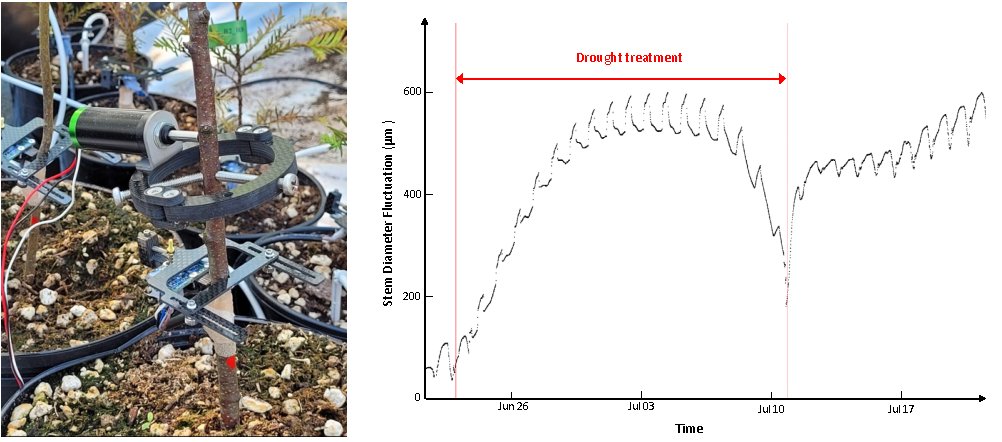
\includegraphics[width=0.8\linewidth, height=0.6\textheight, keepaspectratio]{dendrometer_graph.pdf} 
			\caption{Left: Newly developed magnetic dendrometer (at the stem base) were used to monitor radial growth in a 15 min interval. Their performance was compared to classical point dendrometers (upper part of the stem). Right: Example of the changes in stem diameter of a Bigleaf maple sapling during a drought treatment and subsequent recovery phase.}
			\label{fig:dendrometer_graph}
		\end{figure}
		
	\textbf{Radial cambial growth:}
	The specifically designed magnetic dendrometers performed well and yielded very accurate and comparable results compared to standard point dendrometer (see Fig. \ref{fig:dendrometer_graph}). Measurements during and after drought treatments indicated strong tree water deficits with strong stem shrinkage and almost no recovery during the night (Fig. \ref{fig:dendrometer_graph}). Together with soil moisture measurements this is prove of severe drought conditions. Nevertheless most individuals showed strong recovery after drought stress release. 
	

	
	\textbf{Treatment effects on biomass:}
	Total biomass at the end of the growing seasons was lowest for saplings of all species that were defoliated --- surprisingly even lower than drought-exposed saplings. Although saplings needed a longer recovery from defoliation than from drought stress, Quercus as a fully recovering species that quickly re-flushes from dormant spare buds, showed most reduced biomass compared to control saplings (Fig. \ref{fig:biomass_post_treat_sub}).
	Comparing different timings of drought and defoliation events revealed that biomass accumulation and therefore growth is mostly sensitive to stress around the summer solstice. However, drought had also little effects on biomass just after leaf-out and was negligible in August. Defoliation had even a small positive effect on biomass accumulation in Prunus, Betula and Pinus. Presumably these species were able to compensate later in the season as was observed by a later date of senescence (data not shown here).
	\\
	
	\begin{figure}[H]
		\centering
		\begin{minipage}[t]{0.5\textwidth} % Adjust the width to fit your needs
			\vspace{0pt} % Align the top of minipage with the top of the figure
			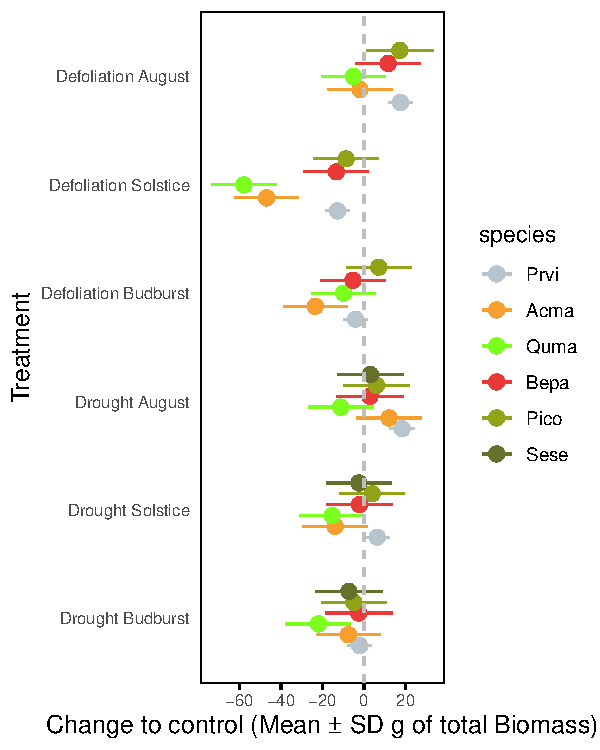
\includegraphics[width=\linewidth, height=0.5\textheight, keepaspectratio]{biomass_post_treat_sub.pdf}
		\end{minipage}%
		\hfill
		\begin{minipage}[t]{0.5\textwidth} % Adjust the width to matc the figure minipage
			\vspace{0pt} % Align the top of minipage with the top of the figure
			\caption{Effect size in g of biomass compared to control sapling when exposed to defoliation or drought treatments on 3 occasions. Colors represent the six study species. Shown are means±SD of the posteriors. Prvi: Prunus; Acma: Acer; Quma: Quercus; Bepa: Betula; Pico: Pinus; Sese: Sequoia.}
			\label{fig:biomass_post_treat_sub}
		\end{minipage}
	\end{figure}

	
	%\textbf{Wood anatomy}
	%Data processing is still under way due to the underestimated time required.
	
		\begin{figure}[H]
		\centering
		\begin{minipage}[t]{0.6\textwidth} % Adjust the width to fit your needs
			\vspace{0pt} % Align the top of minipage with the top of the figure
			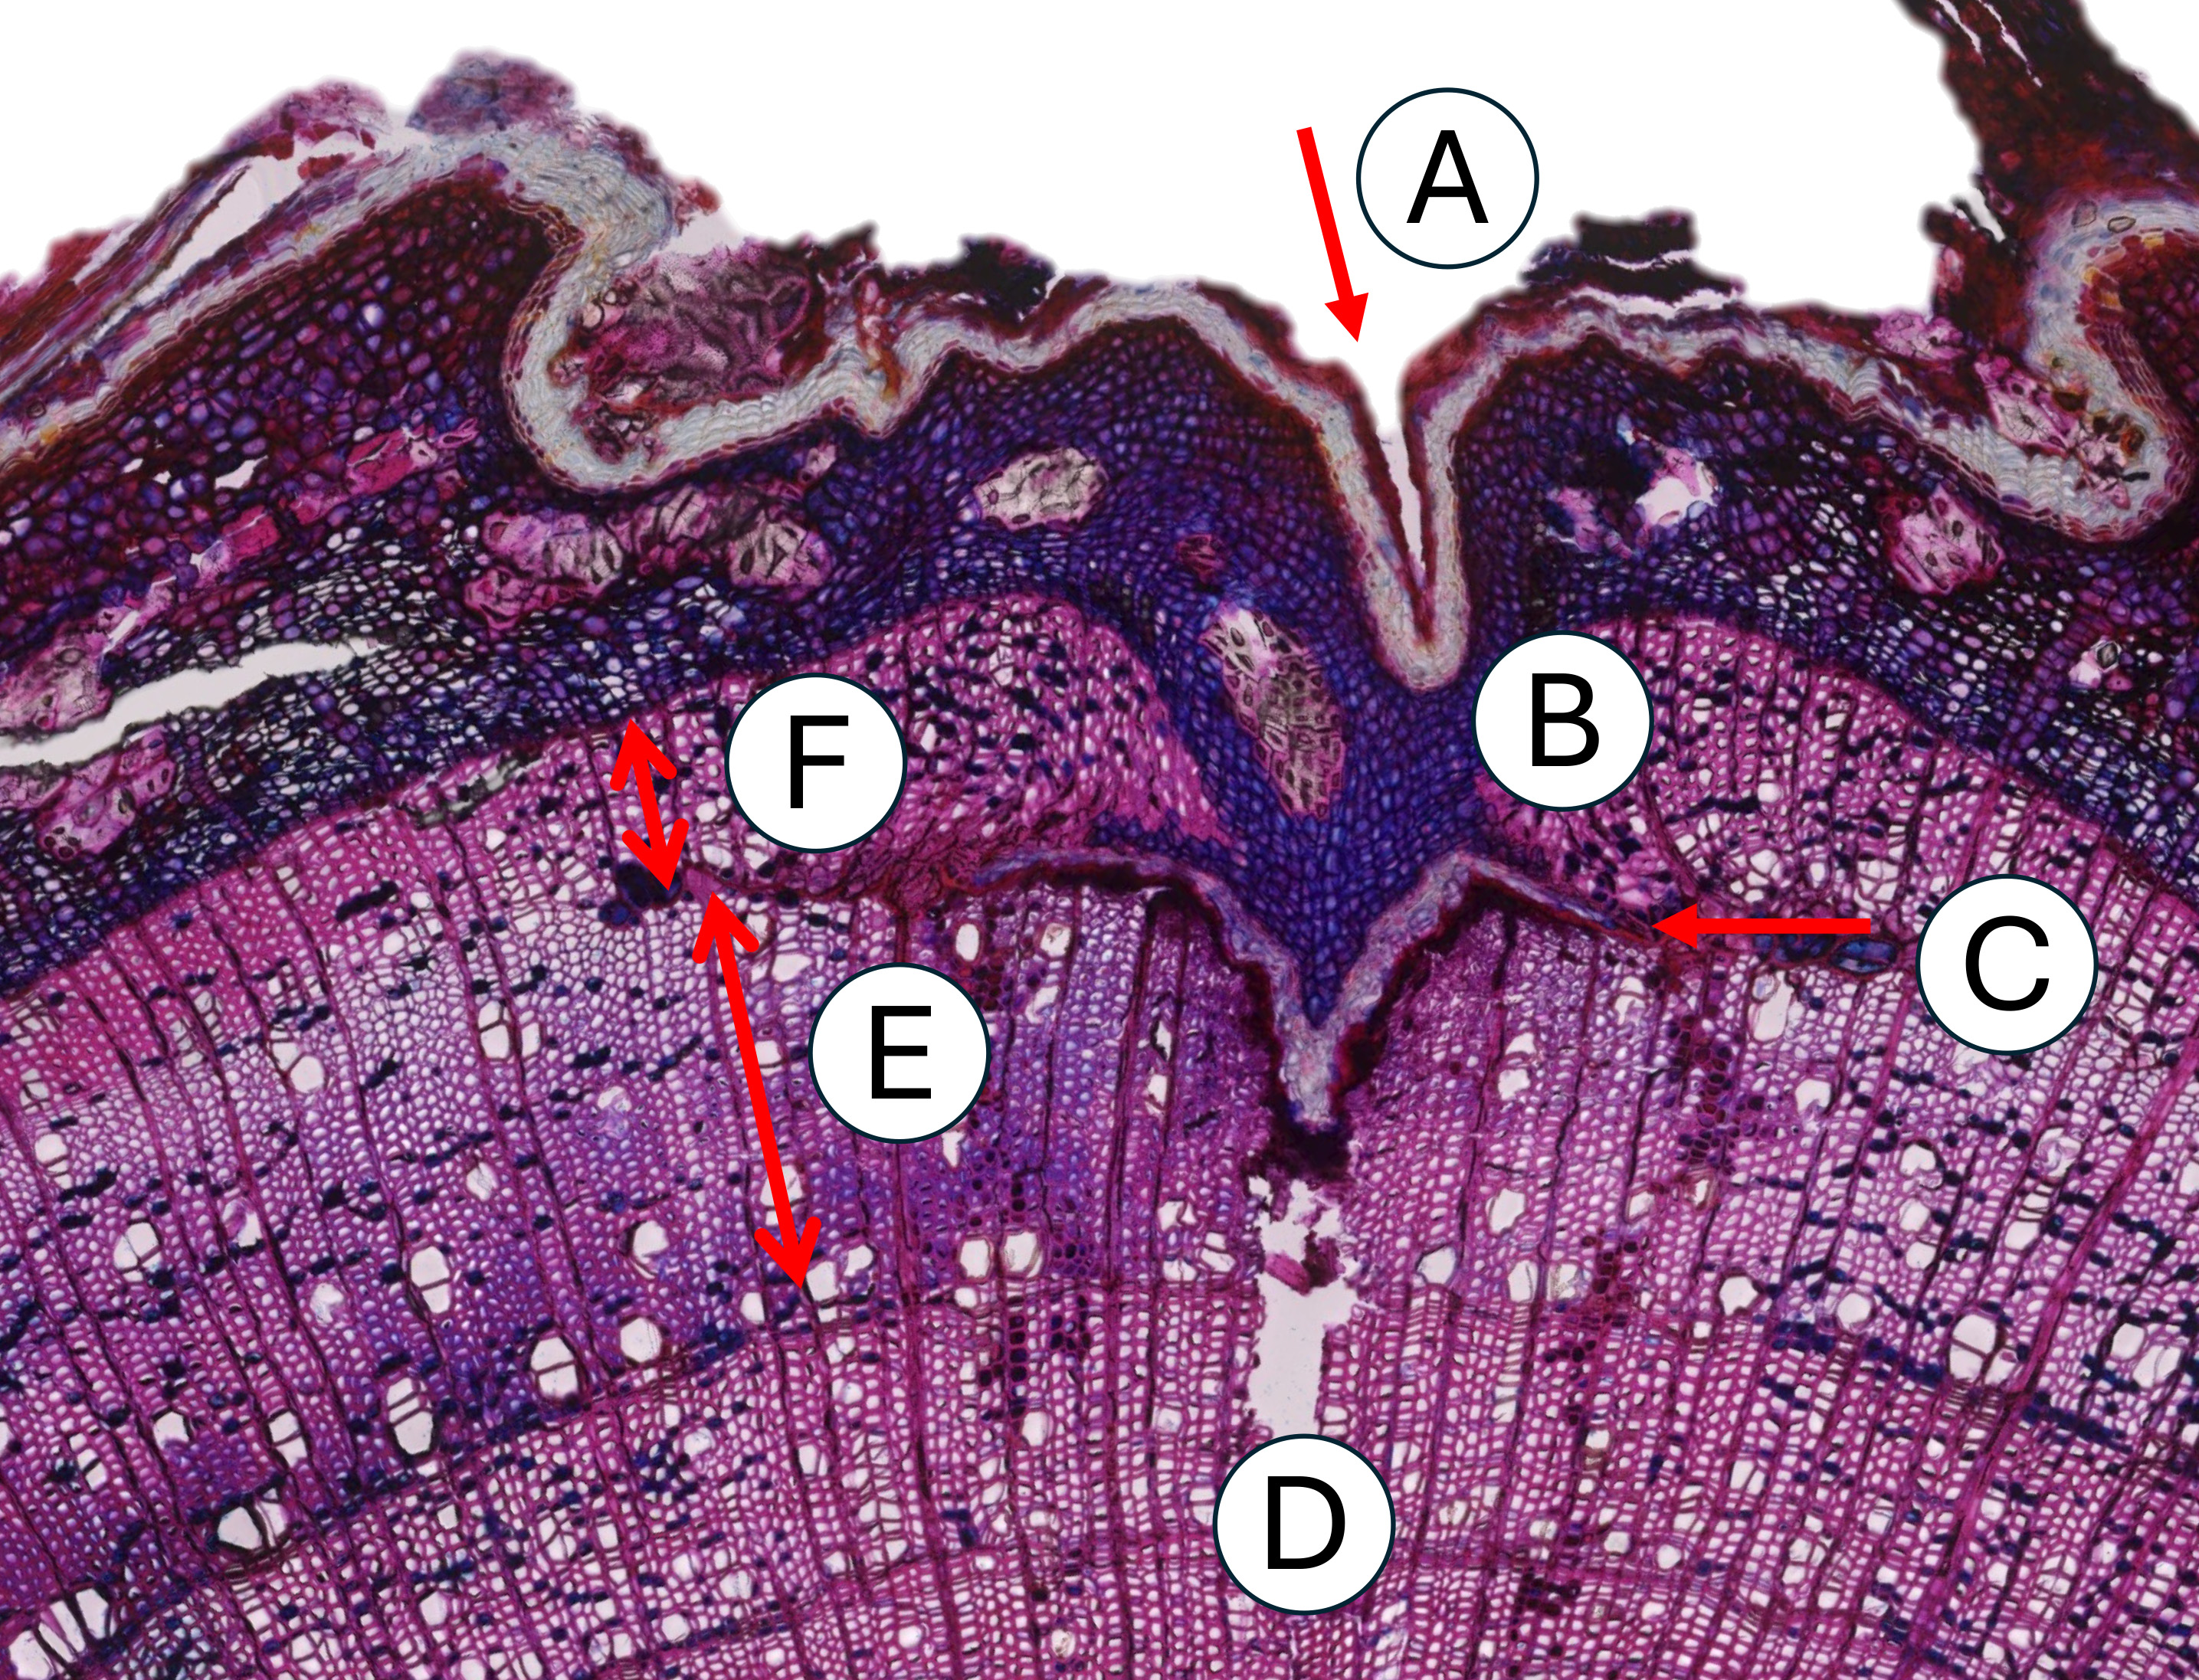
\includegraphics[width=0.8\linewidth, height=0.6\textheight, keepaspectratio]{pinning_closup_x2.jpg}
		\end{minipage}%
		\hfill
		\begin{minipage}[t]{0.4\textwidth} % Adjust the width to matc the figure minipage
			\vspace{0pt} % Align the top of minipage with the top of the figure
			\caption{Cross-section of \textit{Quercus garryana} depicting the reaction caused by the pinning. A: pinning hole with bark and phloem cells; B: zone of irritated cambial cells surrounding the pinning hole (callose tissue); C: border of cambium at the time of pinning; D: Pinning hole penetrating into the xylem cells that were already formed at the time of pinning; E: xylem cells formed prior to pinning; F: xylem cells formed after pinning.}
			\label{fig:pinning_closup_x2}
		\end{minipage}
	\end{figure}
	
	
	
	\section*{Conclusions and outline}
	Preliminary results indicate that defoliation has a stronger negative impact on growth than drought after one growing season. Moreover, effects of stress timing on biomass accumulation matters and is most pronounced in end of June when growth is commonly observed to peak. The pronounced effect of leaf removal, despite fast recovery in most species is surprising because trees are thought to be sink-limited: cell division and maturation are thought to be the most critical and sensitive physiological processes with sugar assimilates often used from reserves. Our data indicate that the formation of new tissue is indeed dependent on fresh assimilates. Moreover, determinate species, that rely on pre-build leaves for the entire season only, appear to be most affected from defoliation events. Indeterminate growing species, in contrast, may compensate stress episodes by prolonging or shifting their growth phenology. Such a phenotypic plasticity may become crucial in a climate with increased frequency of environmental stress and should be further investigated as an important functional trait.\\
	
	Our results also emphasize that the effects of environmental stress may not become apparent in the current year but could rather manifest in the subsequent year. Determinate species, in particular, are likely to experience reduced performance in the following year, as their entire next year's foliage is formed in the current year, eventually under poor conditions. This in turn may largely define the growth potential  in the upcoming year.\\
	
	Depending on how much tissue is pre- versus neo-formed in a current growing season, species may perform differently under environmental stress. This finding has inspired two follow-up projects: 1) a literature search was launched to review the concept of (in)determinism and to screen species for their degree of indeterminism. 2) an experiment was launched to investigate how warming in spring and/or autumn affects growth performance not only in the current but also in the following year (carry over effect). Part of this work was presented at ESA, Longbeach, CA and EGU, Vienna. 
	

	
	
	
	
	
	
	
	
	%\section*{stuff I did't find place yet}
	
	

	
	
	\bibliography{refs_phaenoflex}
	\bibliographystyle{ecolett}
	
	
	
	
	
	
\end{document}
